\chapter{Diseño e Implementación} % Main chapter title

\label{Chapter3} % Change X to a consecutive number; for referencing this chapter elsewhere, use \ref{ChapterX}
\definecolor{mygreen}{rgb}{0,0.6,0}
\definecolor{mygray}{rgb}{0.5,0.5,0.5}
\definecolor{mymauve}{rgb}{0.58,0,0.82}

\lstset{ %
  backgroundcolor=\color{white},   % choose the background color; you must add \usepackage{color} or \usepackage{xcolor}
  basicstyle=\footnotesize,        % the size of the fonts that are used for the code
  breakatwhitespace=false,         % sets if automatic breaks should only happen at whitespace
  breaklines=true,                 % sets automatic line breaking
  captionpos=b,                    % sets the caption-position to bottom
  commentstyle=\color{mygreen},    % comment style
  deletekeywords={...},            % if you want to delete keywords from the given language
  %escapeinside={\%*}{*)},          % if you want to add LaTeX within your code
  %extendedchars=true,              % lets you use non-ASCII characters; for 8-bits encodings only, does not work with UTF-8
  %frame=single,	                   % adds a frame around the code
  keepspaces=true,                 % keeps spaces in text, useful for keeping indentation of code (possibly needs columns=flexible)
  keywordstyle=\color{blue},       % keyword style
  language=[ANSI]C,					% the language of the code
  %otherkeywords={*,...},           % if you want to add more keywords to the set
  numbers=left,                    % where to put the line-numbers; possible values are (none, left, right)
  numbersep=5pt,                   % how far the line-numbers are from the code
  numberstyle=\tiny\color{mygray}, % the style that is used for the line-numbers
  rulecolor=\color{black},         % if not set, the frame-color may be changed on line-breaks within not-black text (e.g. comments (green here))
  showspaces=false,                % show spaces everywhere adding particular underscores; it overrides 'showstringspaces'
  showstringspaces=false,          % underline spaces within strings only
  showtabs=false,                  % show tabs within strings adding particular underscores
  stepnumber=1,                    % the step between two line-numbers. If it's 1, each line will be numbered
  stringstyle=\color{mymauve},     % string literal style
  tabsize=2,	                   % sets default tabsize to 2 spaces
  title=\lstname,                   % show the filename of files included with \lstinputlisting; also try caption instead of title
  morecomment=[s]{/*}{*/}%
}


%----------------------------------------------------------------------------------------
%	SECTION 1
%----------------------------------------------------------------------------------------
En este capítulo se presenta cómo se desarrolló el hardware básico para simular el entorno de funcionamiento y cómo fue implementado el firmware.
%La idea de esta sección es resaltar los problemas encontrados, los criterios utilizados y la justificación de las decisiones que se hayan tomado.
%Se puede agregar código o pseudocódigo dentro de un entorno lstlisting con el siguiente código:

\section{Hardware}

Primeramente se diseñó un circuito electrónico que permite simular el entorno de funcionamiento de una bodega. Para ello se utilizó lo aprendido a la largo del curso de \emph{diseño de PCBs en KICAD}. 

En la figura \ref{fig:diagrama_sistema} se aprecia el entorno de trabajo del sistema. El mismo interactua con una bomba de agua que permite llevar liquido refrigerante desde el depósito hacia los tanques que están en proceso de fermentación.
Recibiendo como información la temperatura de los tanques, el equipo debe controlar la bomba y la electroválvula correspondiente. De esta forma se controla la temperatura acorde a los parámetros definidos por el usuario. 


\begin{figure}[!htb]
  \centering
  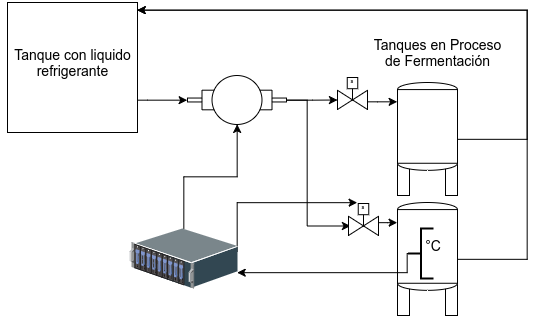
\includegraphics[scale=0.7]{./Figures/diagrama_del_sistema.png}
  \caption{Entorno del sistema de control del equipo.}
  \label{fig:diagrama_sistema}
\end{figure}

\subsection{ Módulos requeridos}
Para llevar a cabo el proyecto, se dividió el sistema en los siguientes módulos:
\begin{description}
  \item[Módem:] encargado de transmitir las alertas mediante SMS utilizando el modulo SIM800L.
  \item[Actuadores:] salidas que permiten controlar la bomba y electroválvulas.
  \item[Sensores:] entradas que permitan simular el comportamiento de los sensores, para esto se utilizaron potenciómetros.
  \item[CPU:] unidad encargada de controlar el funcionamiento del sistema incorporada en la placa CIAA-NXP. 
\end{description}

\subsection{Características del hardware}

Como se vió en la figura \ref{fig:diagrama_sistema} el dispositivo de monitoreo interactua con la temperatura de los tanques, el control de la bomba y la seleccion de la electrovalvula. Es por esto que se implementó un sitema que está compuesto por el modem y circuitos electronicos que permiten:
\begin{itemize}
  \item Simular el estado de la temperatura
  \item Adaptar los niveles de tensión.
  \item Mostrar el estado de los actuadores.
  \item Conectar el módem GPRS.
\end{itemize}

    De esta forma la placa desarrollada la cual llamaremos simulador del sistema, nos permite conectar el modem y validar el correcto funcionamiento del software implementado. La forma de conexión con la CIAA-NXP se muesetra en la figura \ref{fig:diagrama_simulado}.

\begin{figure}[!htb]
  \centering
  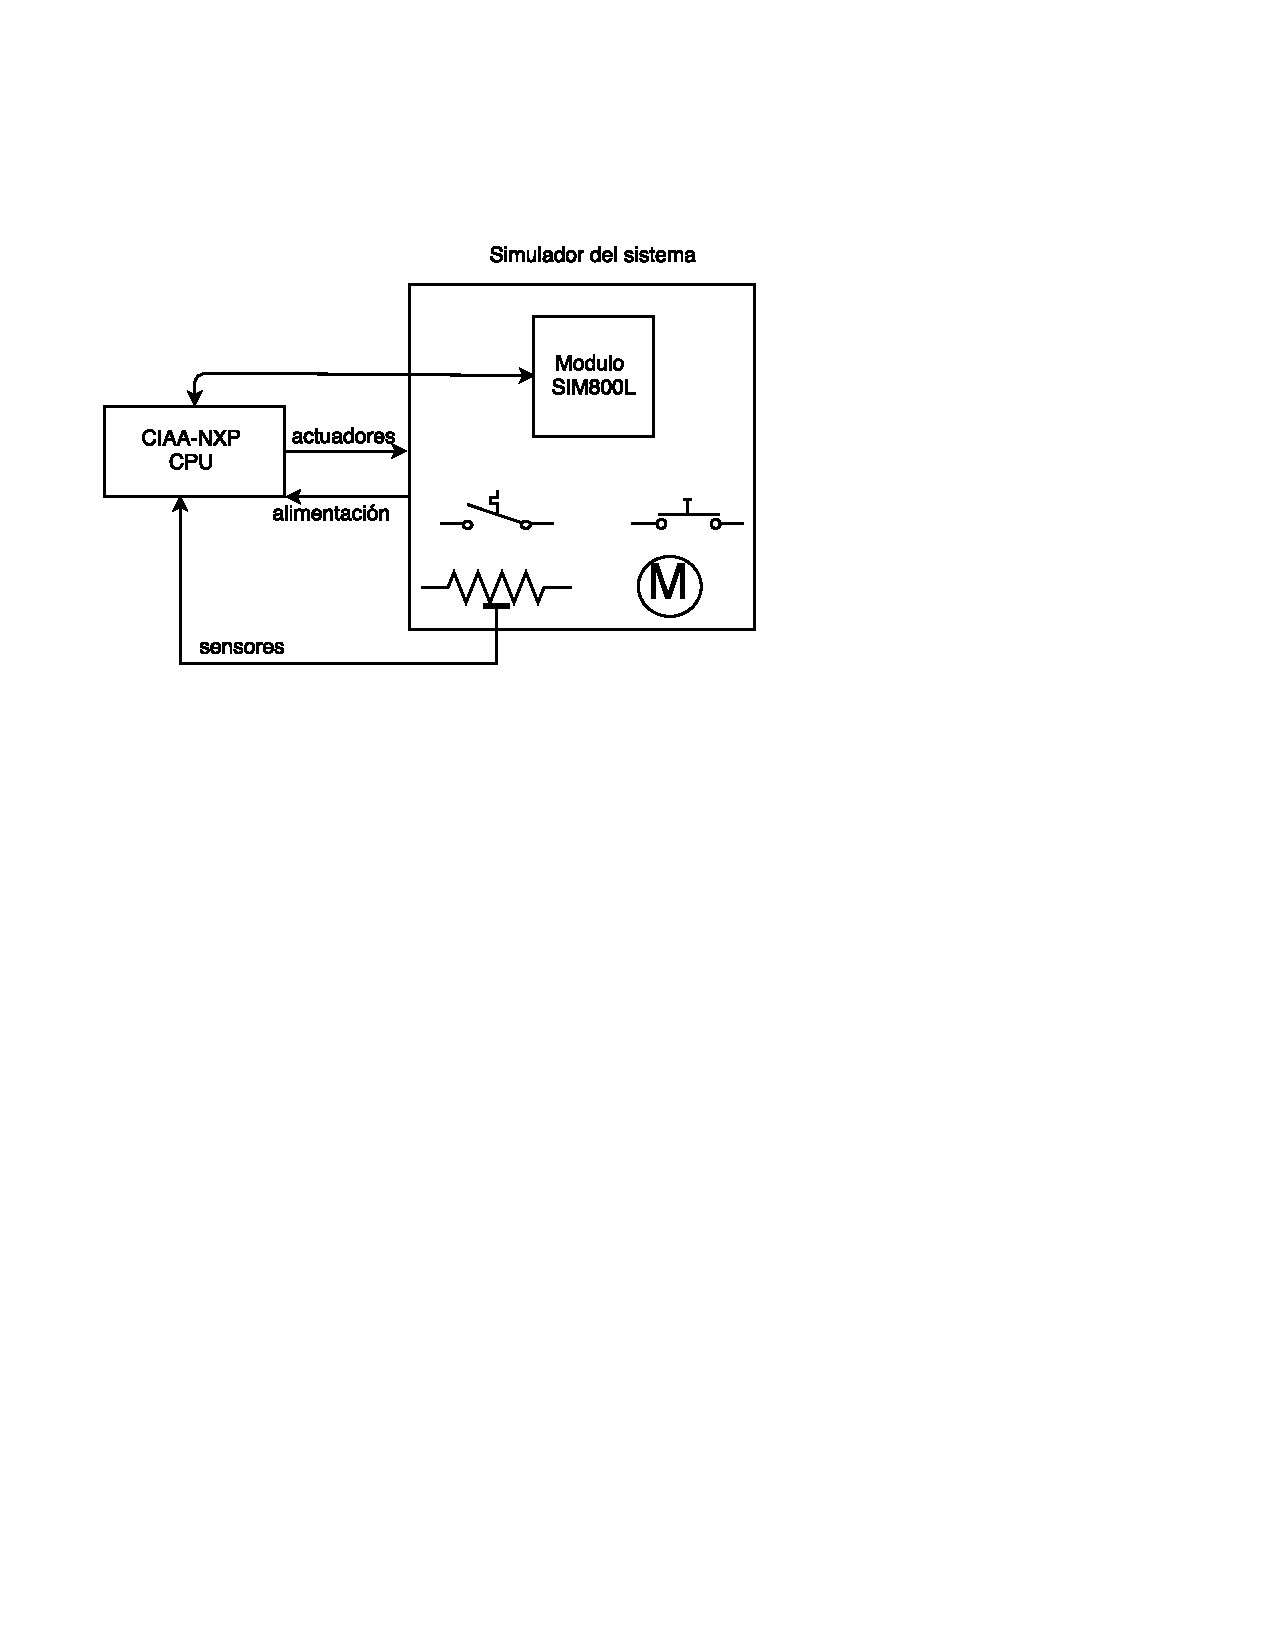
\includegraphics[page=1,scale=1,clip,trim=1.5cm 16.5cm 5.5cm 3.5cm]{./Figures/ciaa_placa_base.pdf}
  \caption{Conexion de la CIAA-NXP con el simulador del sistema.}
  \label{fig:diagrama_simulado}
\end{figure}


La placa de simulación debe contar con las siguientes entradas, salidas y zócalos:

\begin{itemize}
  \item 1 Salida con regulación de corriente, para simular sensores de 4mA a 20mA.
  \item 3 Salida de tensión variable.
  \item 1 Salida de sensor de temperatura LM35.
  \item 4 Entradas digitales conectadas a leds.
  \item 4 Salidas conectadas a pulsadores. 
  \item 1 Zócalo para la conexión del modulo SIM800L. 
  \item 1 salida de 5V a 3A y otra de 3.3V a 1A. 
\end{itemize}

El módulo SIM800L se muestra en la figura \ref{fig:sim800l} y es un módem GPRS que cuenta con las siguientes especificaciones:

\begin{figure}[!htb]
  \centering
  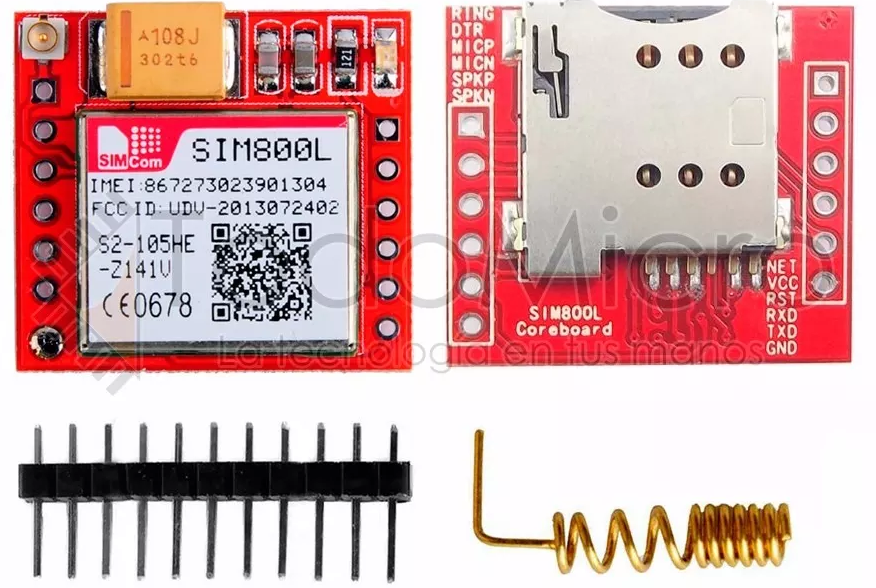
\includegraphics[scale=0.2]{./Figures/sim800.png}
  \caption{Módem SIM800L.}
  \label{fig:sim800l}
\end{figure}

\begin{itemize}
  \item Alimentación: 3.4V a 4.4V (4.0V recomendado)
  \item  CuatriBanda 850/900/1800/1900MHz
  \item  GPRS Multi Slot class 8/10
  \item  Control mediante comandos AT (GSM 07.07 ,07.05 y comandos AT SIMCOM).
\end{itemize}


En la figura \ref{fig:essim800} se aprecia el esquemático implementado para la conexión del módem GSM. Éste requiere adaptar los niveles de tensión para interactuar con la CIA-NXP, para el cual se utilizó el max3232.
\begin{figure}[!hp]
  \centering
  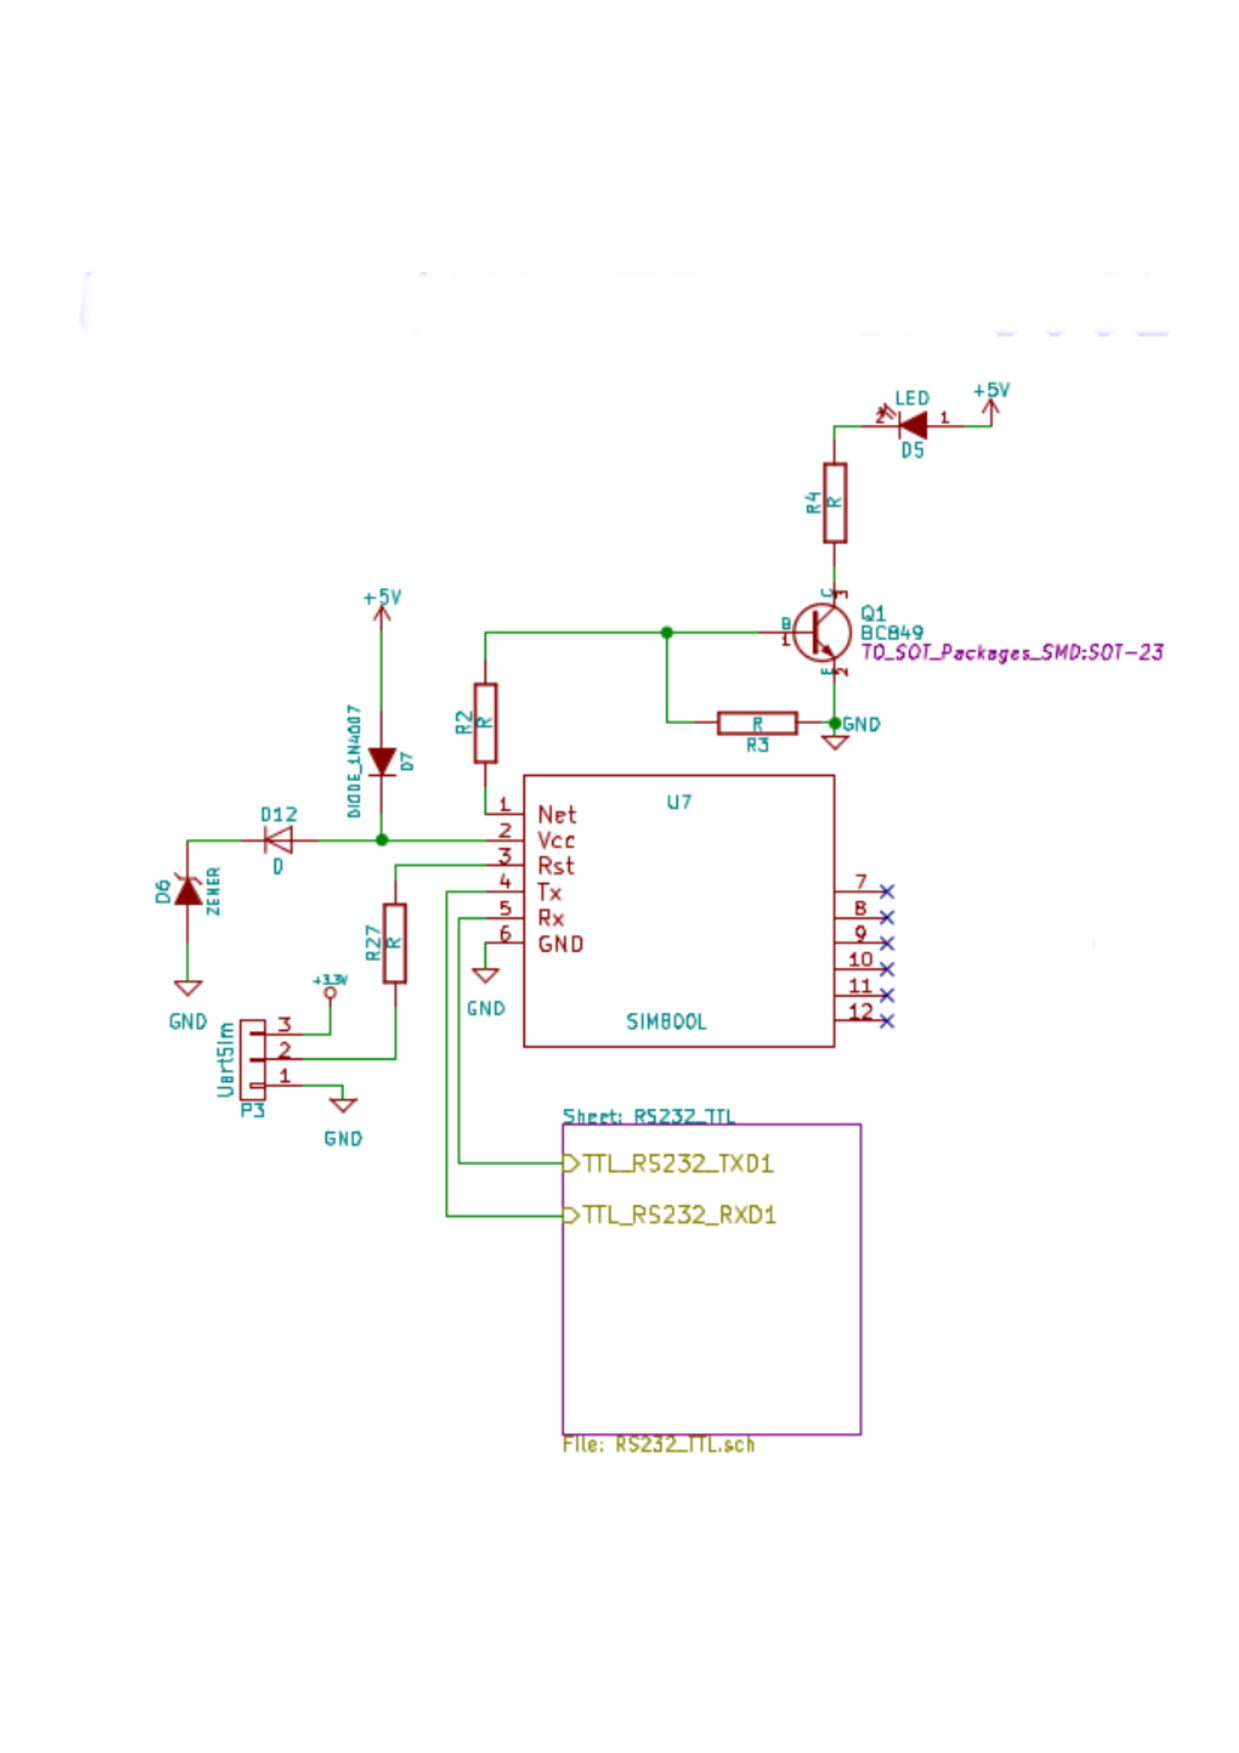
\includegraphics[page=1,scale=0.5,clip,trim=1cm 4.7cm 1.2cm 6.5cm]{./Figures/sch_modem_sim800.pdf}
  \caption{Circuito de conexión del módulo SIM800l.}
  \label{fig:essim800}
\end{figure}

Para la alimentación del circuito se utilizó el regulador LM2576. El mismo se tomó de la nota de aplicación \citep{Texas:LM2576}.
Y para regular a 3.3V se utilizó el integrado LM11733 circuito extraído de la nota de aplicación \citep{Texas:LM11733}. El esquemático se aprecia en la figura: \ref{fig:fuente}.
\begin{figure}[!hp]
  \centering
  \includegraphics[page=3,scale=0.7,angle=270,clip,trim=5cm 3cm 6.5cm 2.5cm]{./Figures/schematic.pdf}
  \caption{Fuente de alimentación DC/DC.}
  \label{fig:fuente}
\end{figure}

Para lograr la simulación de distintos tipos de sensores, se utilizaron circuitos como el que se muestra en la figura \ref{fig:sch_ireg}  que permiten generar corrientes de 4mA a 20mA.
También reguladores de tensión, vease en la figura \ref{fig:sch_vreg} y un sensor de temperatura en la figura \ref{fig:sch_lm35}. Para estos circuitos se utilizaron las notas de aplicación de Texas Instruments\citep{Texas:LM317} - capitulo 8 páginas 12 y 13 y sensor temperatura: \citep{Texas:LM35} - 8.2.1 Basic Centigrade Temperature Sensor. 
\begin{figure}[!hp]
  \centering
  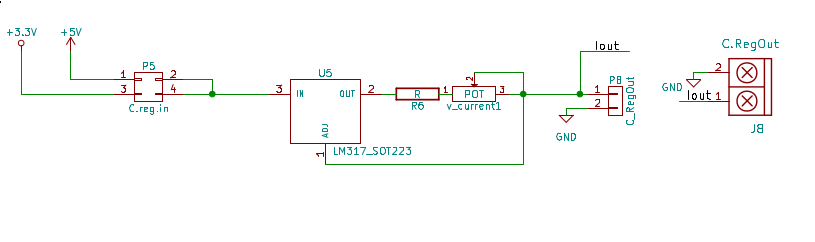
\includegraphics[scale=0.5]{./Figures/sch_ireg.png}
  \caption{Circuito regulador de corriente.}
  \label{fig:sch_ireg}
  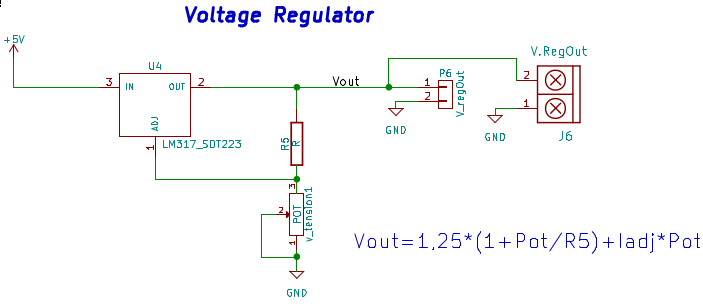
\includegraphics[scale=0.5]{./Figures/sch_vreg.png}
  \caption{Circuito regulador de tensión.}
  \label{fig:sch_vreg}
  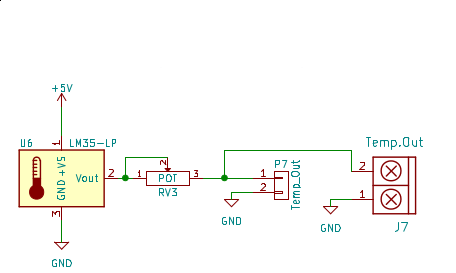
\includegraphics[scale=0.5]{./Figures/sch_lm35.png}
  \caption{Circuito del sensor de temperatura.}
  \label{fig:sch_lm35}
\end{figure}

Para concluir, se utilizaron circuitos básicos que permiten interactuar en forma simple con el sistema y realizar pruebas de funcionamiento.
Los mismos fueron extraídos del esquemático utilizado en el proyecto de la EDU-CIA \footnote{\url{http://www.proyecto-ciaa.com.ar/devwiki/lib/exe/fetch.php?media=desarrollo:edu-ciaa:edu-ciaa-nxp:edu-ciaa-nxp\_color.pdf}}, figura \ref{fig:pul_leda_pulses}.


\begin{figure}[!hp]
  \begin{subfigure}{0.4\textwidth}
    \centering
    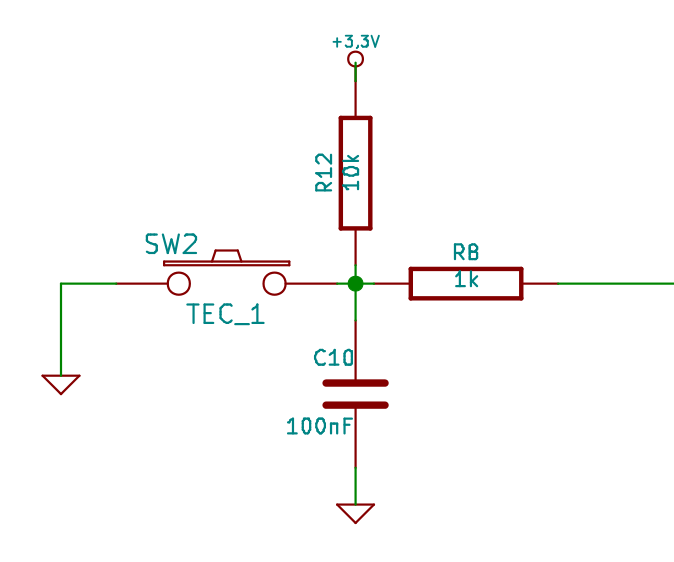
\includegraphics[width=1\linewidth]{./Figures/pulse_sch.png}
    \caption{Circuito de los pulsadores.}
  \end{subfigure}%
  \hfill
  \begin{subfigure}{0.4\textwidth}
    \centering
    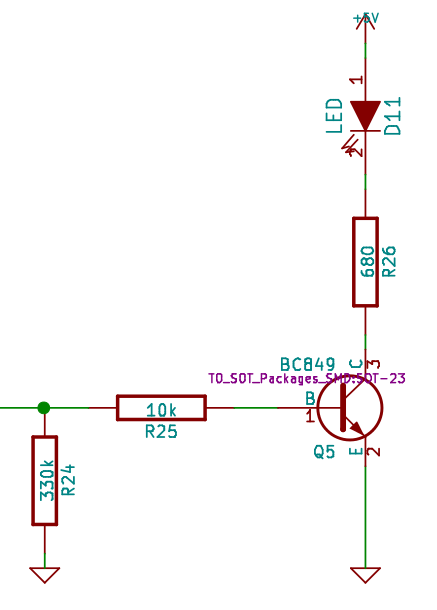
\includegraphics[width=1\linewidth]{./Figures/led_sch.png}
    \caption{Circuito de los leds.}
  \end{subfigure}
  \caption{Esquematicos extraidos de la EDU-CIAA.}
  \label{fig:pul_leda_pulses}
\end{figure}

Con los esquemáticos terminados, se pasó a la elaboración del circuito impreso que se presentan en las figuras \ref{fig:layer_sup}, \ref{fig:layer_inf} y \ref{fig:pcb3d}.
\begin{figure}[!hp]
  \centering
  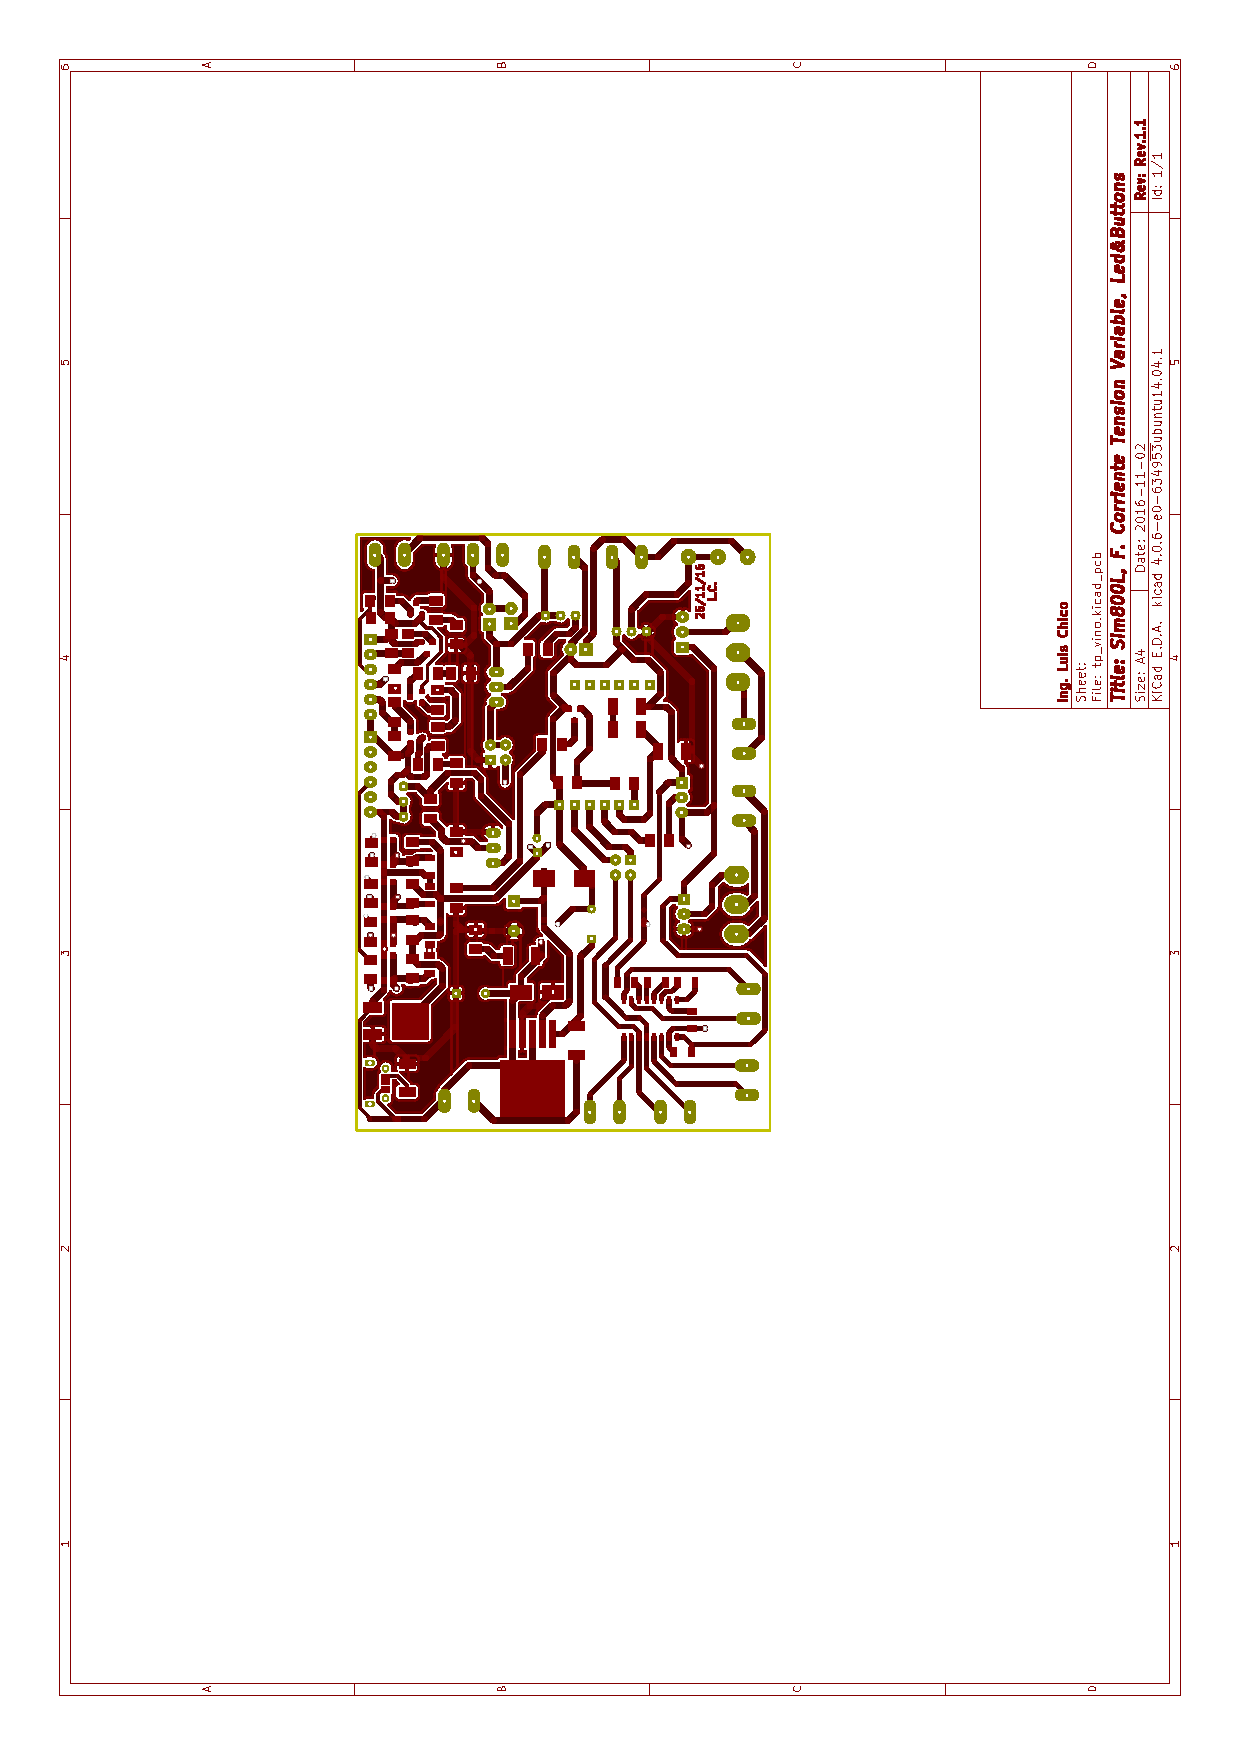
\includegraphics[page=1,angle=270,clip,trim=5.5cm 10cm 7.7cm 8.5cm]{./Figures/pcb_layer.pdf}
  \caption{Capa superior de la placa de simulación de sensores.}
  \label{fig:layer_sup}
\end{figure}
\begin{figure}[!hp]
  \centering
  \includegraphics[page=2,angle=270,clip,trim=5.5cm 10cm 7.7cm 8.5cm]{./Figures/pcb_layer.pdf}
  \caption{Capa inferior de la placa de simulación de sensores.}
  \label{fig:layer_inf}
\end{figure}

\begin{figure}[!hp]
  \centering
  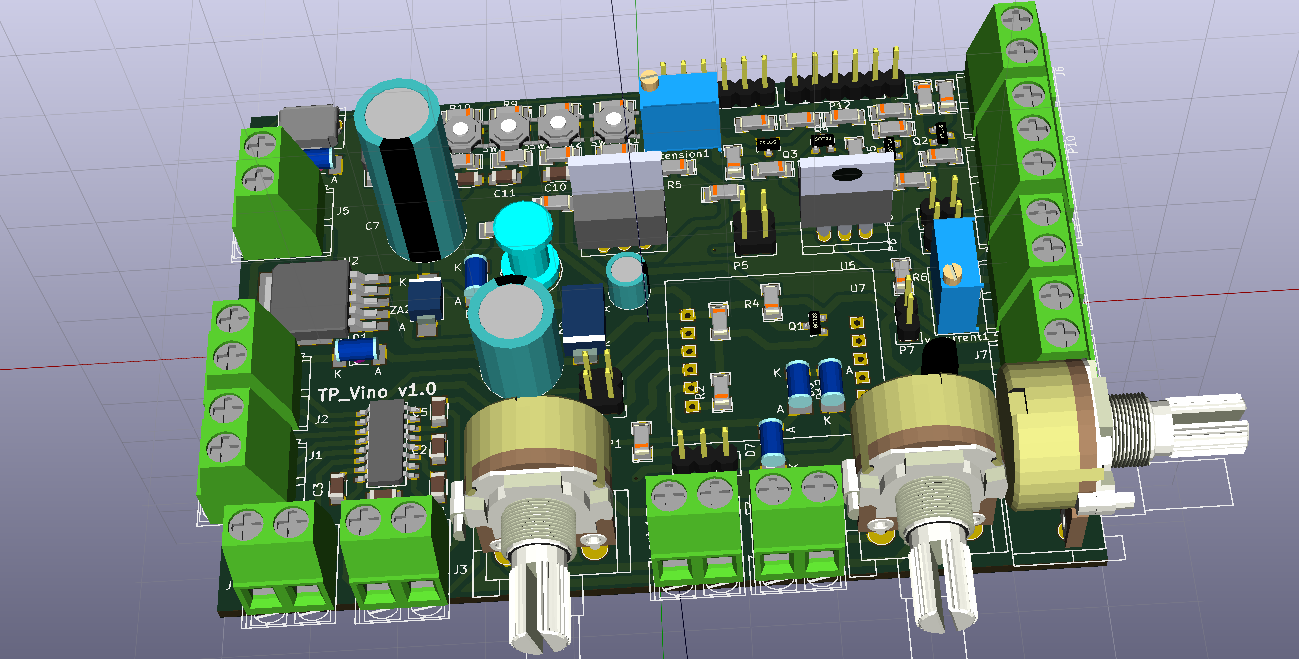
\includegraphics[scale=0.3]{./Figures/pcb_3d.png}
  %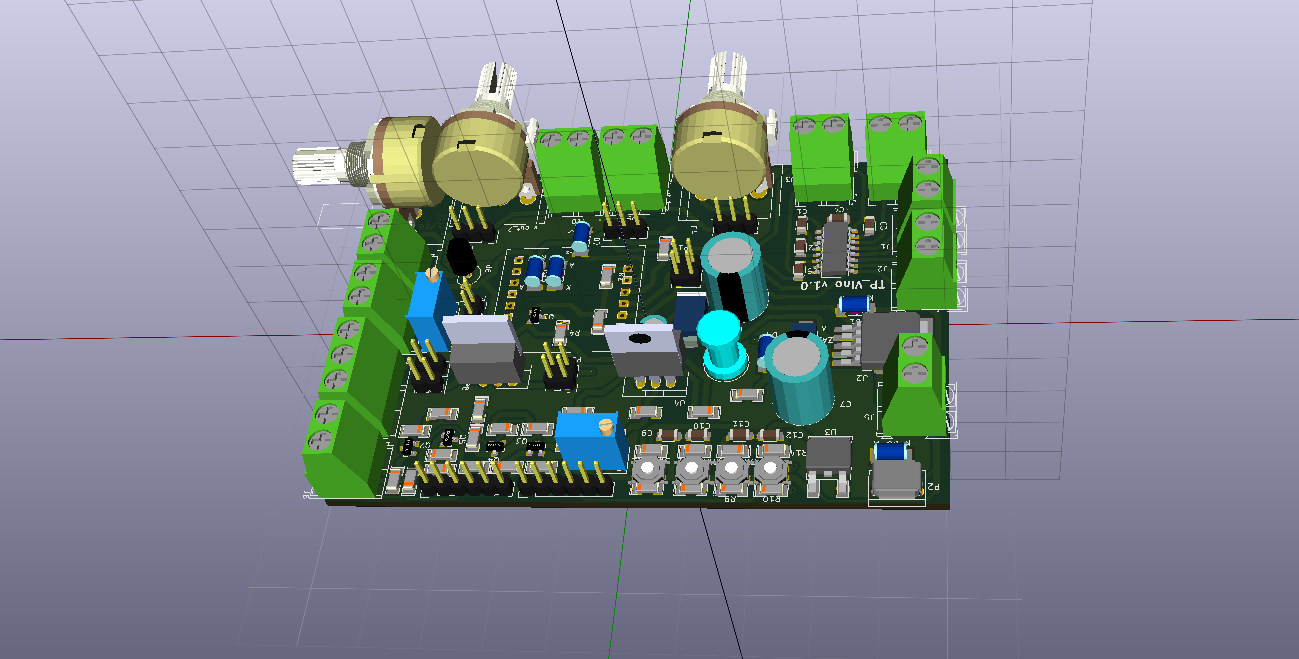
\includegraphics[scale=0.3]{./Figures/pcb_3d_back.png}
  \caption{Placa simulador de sensores 3D.}
  \label{fig:pcb3d}
\end{figure}

No obstante, por cuestiones de tiempo no se llegó a implementar la placa que se diseñó del simulador del sistema y se terminó desarrollando una placa experimental que se presenta en la figura \ref{fig:placa_básicafirst}, la cual permitió realizar las primeras pruebas.

\begin{figure}[!ht]
  \centering
  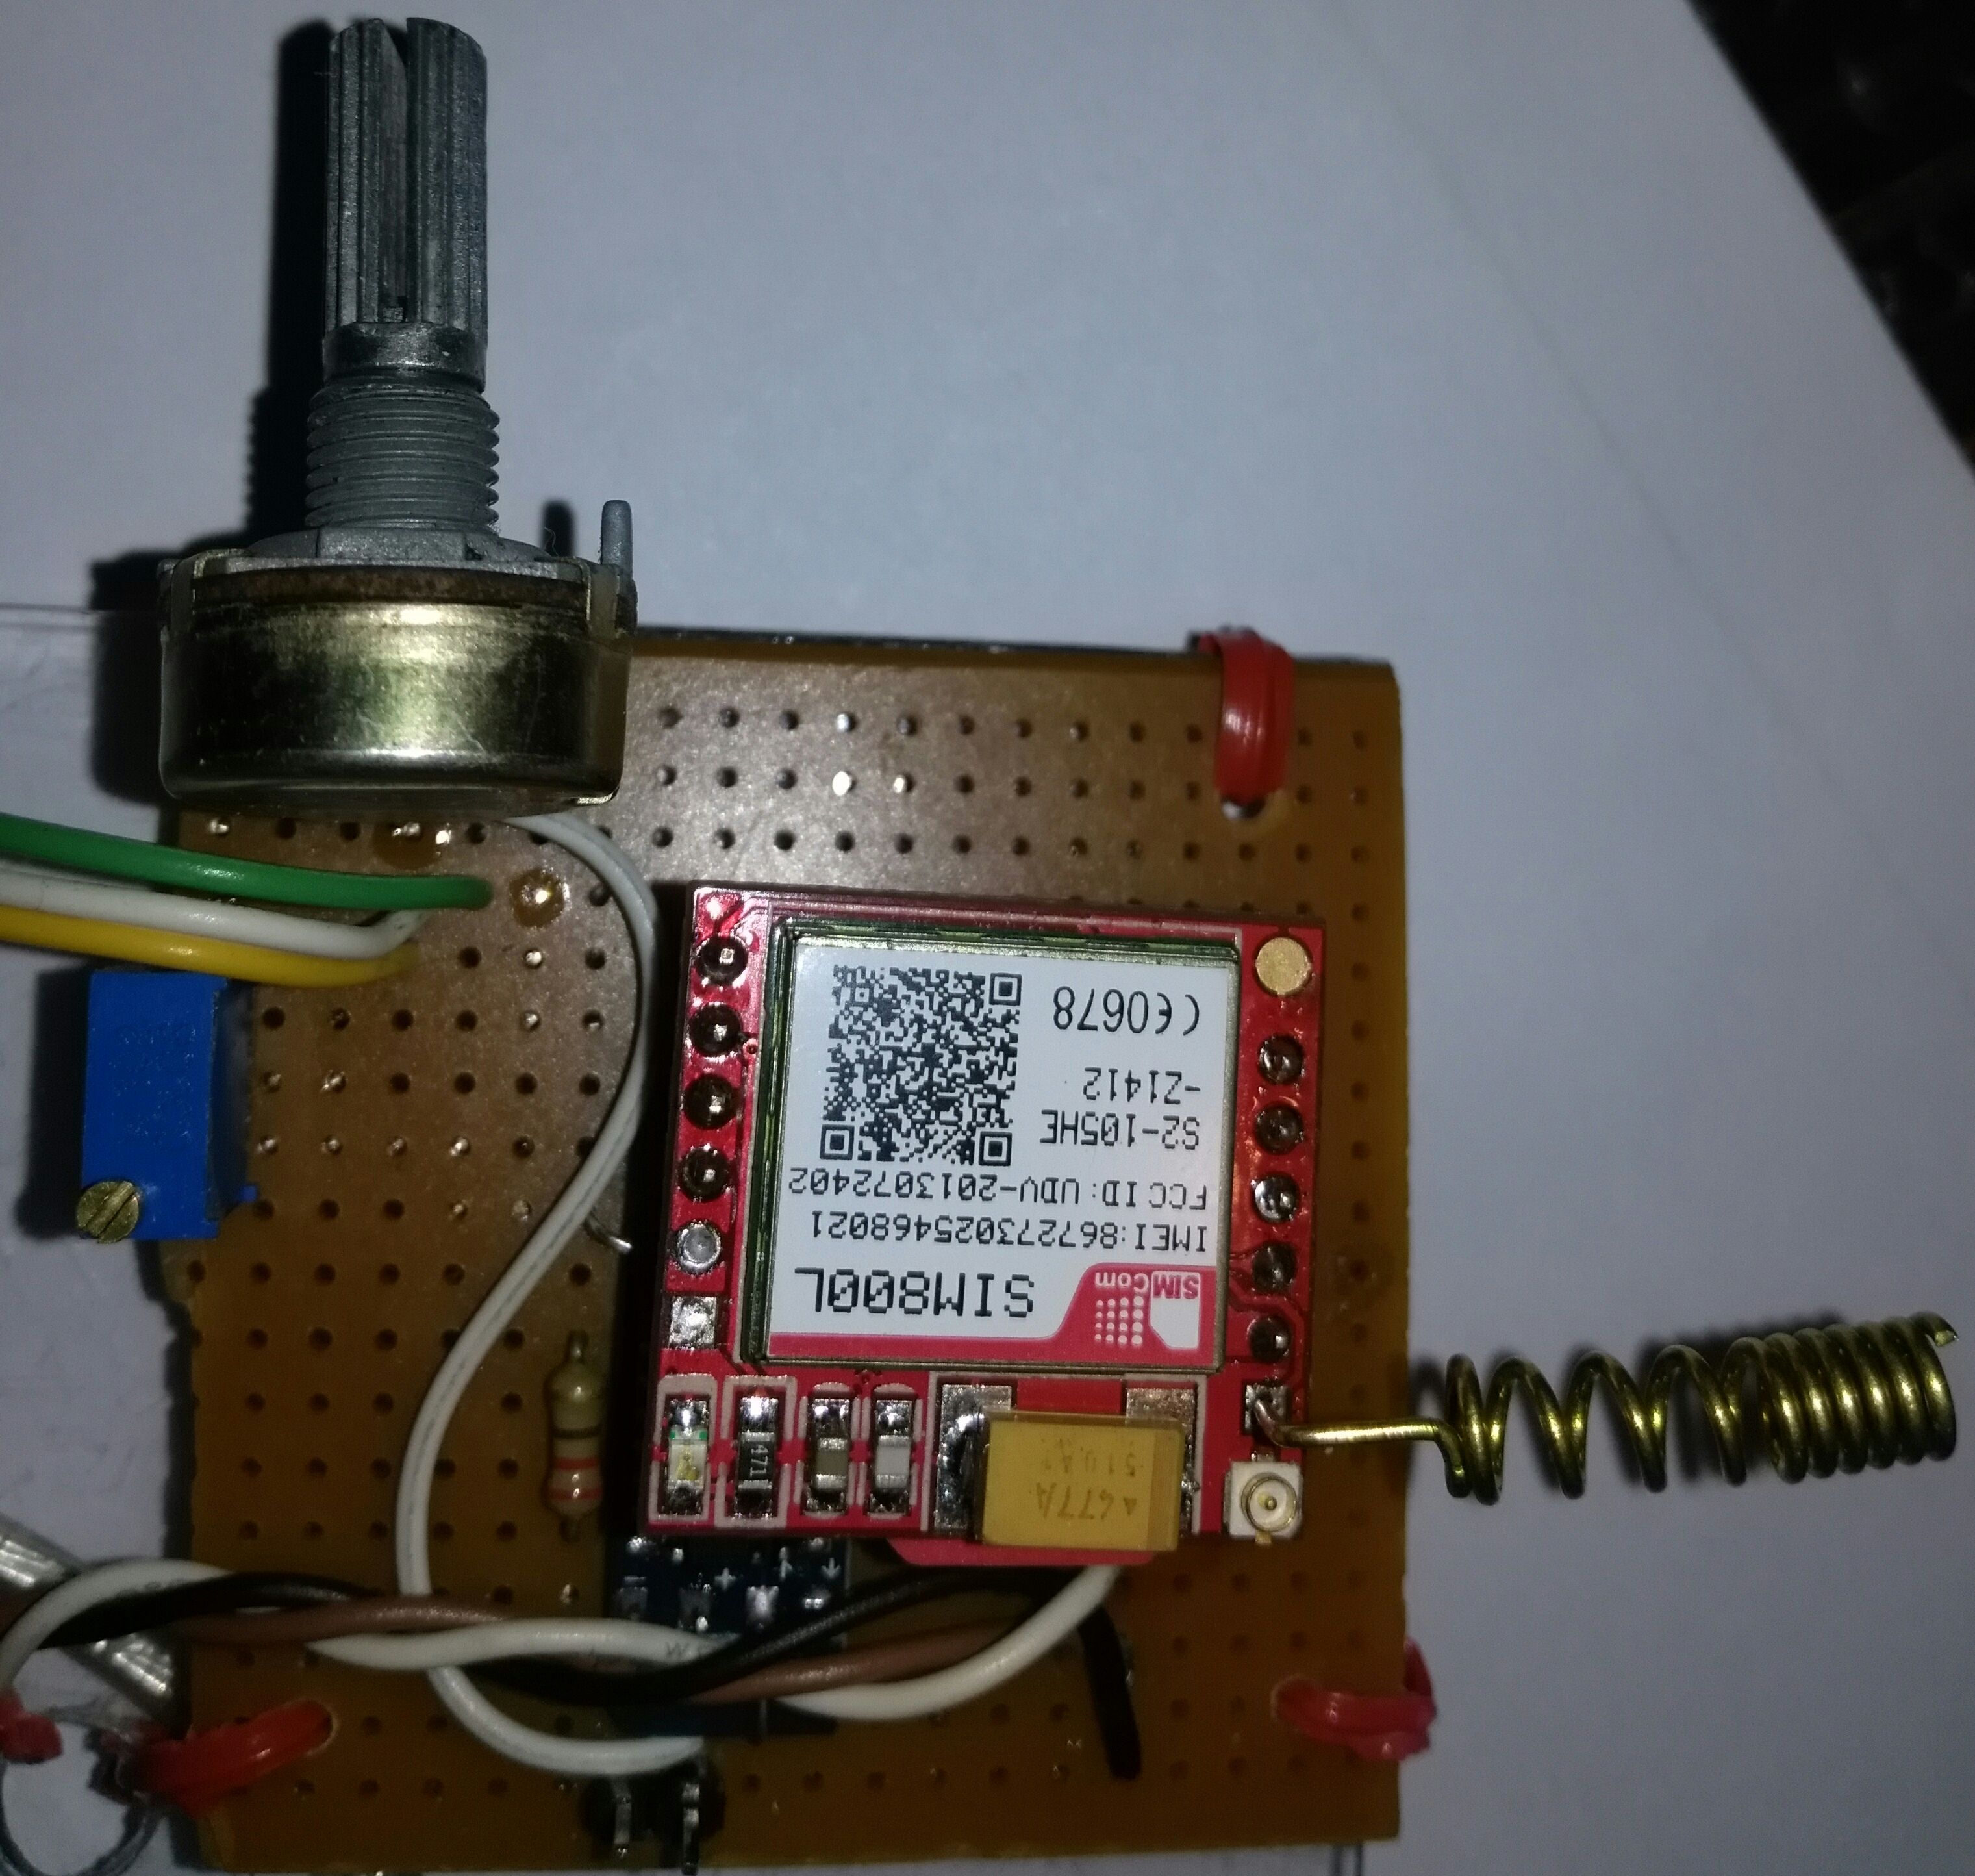
\includegraphics[scale=.07]{./Figures/placa_basica.jpg}
  \caption{Placa de simulación de temperatura y estado de la batería con el modulo SIM800L integrado.}
  \label{fig:placa_básicafirst}
\end{figure}


%Dado que por falta de tiempo no se elaboro el PCB diseñado, pero se realizó una versión simplificada del mismo que se verá más adelante. 
%
%Surgieron varios imprevistos, principalmente con el modulo SIM800L, el cual posee grandes inconvenientes a la hora de detectar la SIM. Luego de una serie de búsquedas en internet, donde muchos habían tenido un problema similar dado que:
%\begin{itemize}
%  \item La fuente de alimentación fue subdimensionada.
%  \item Módulo es muy sensible y se debe limpiar bien los contactos de la SIM.
%  \item O problemas con las soldaduras del módulo.
%\end{itemize}
%Finalmente, como el módulo ya había sido comprado y se encontró la falla a tiempo, se utilizó este en el prototipo.
%Pero este no se recomienda por los problemas mencionados anteriormente. A futuras implementación este módulo será reemplazado.




\section{Software}
\subsection{Aplicación}
Para la implementacion de la lógica del sistema se dividieron en tres tareas: módem, control y sensores. 

\subsection*{Sensor}

Esta consulta el estado de los sensores y calcula el promedio de las ultimas N muestras. Este es el valor que utiliza la tarea de control para definir si es necesario encender los actuadores correspondientes o apagarlos.

El diagrama de flujo se puede apreciar en la figura \ref{fig:sensor_task}.

\begin{figure}[!htp]
  \centering
  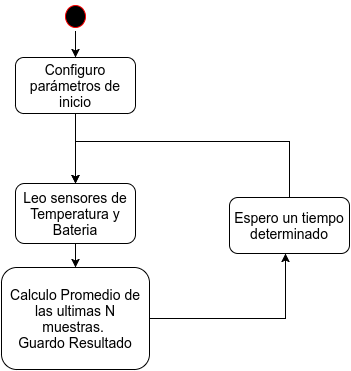
\includegraphics[scale=.7]{./Figures/sensor_task.png}
  \caption{Diagrama de flujo de la tarea sensor.}
  \label{fig:sensor_task}
\end{figure}


\subsection*{Módem}
  En esta tarea se inicializa las configuraciones iniciales para el uso del módem. El cual requiere que esté configurado en modo texto para poder transmitir mensajes SMS. A su vez, es la encargada de interactuar con el módulo GPRS realizando consultas del nivel de señal del módem y de enviar los mensajes de alarmas si estas estan activadas y son necesarias.

  En el diagrama de flujo se aprecia en la figura \ref{fig:modem_task}.

  \begin{figure}[!htp]
    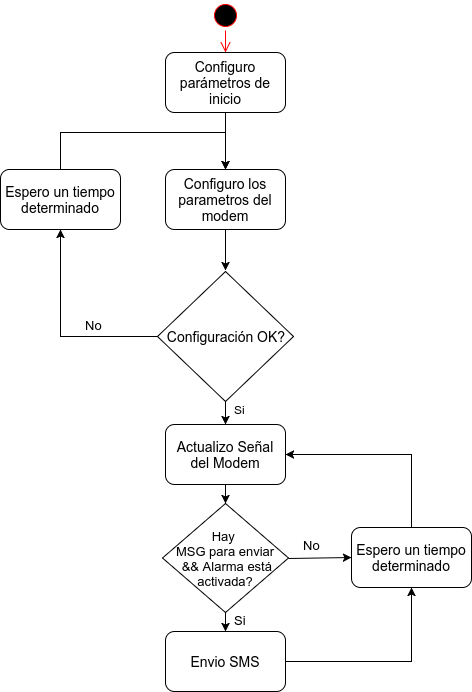
\includegraphics[scale=.7]{/Figures/modem_task.png}
    \caption{Diagrama en flujo de la tarea modem}
    \label{fig:modem_task}
\end{figure}


\subsection*{Control}
La tarea de control es la que:
  
\begin{itemize}
  \item Analiza los resultado de los sensores de temperatura y de la batería verificando que estén dentro de los parámetros configurados por el usuario y actúa en consecuencia. Si la temperatura del sistema excede la máxima configurada y el control automático esta activado entonces esta procede a encender la bomba y activar la electroválvula para que circule el líquido refrigerante por el tanque correspondiente. Luego una vez que la temperatura baja hasta la mínima, este deshabilita la bomba y la electroválvula. De no estar activado el control automático, la bomba y la electroválvula continúan en el estado que estaban, es decir no se realiza ninguna acción.
  \item Es la encargada de setear los actuadores según sean especificados en la plataforma web.
\end{itemize}

El diagrama de flujo correspondiente se puede apreciar en la figura \ref{fig:control_task}.
\begin{figure}[hp]
  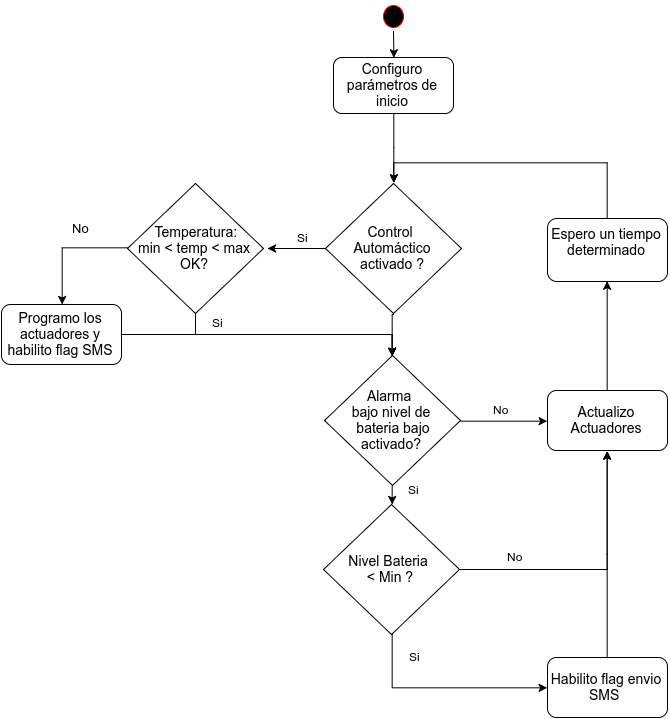
\includegraphics[scale=.5]{./Figures/control_task.png}
  \caption{Diagrama de flujo de la tarea control.}
  \label{fig:control_task}
\end{figure}


\subsection{ Plataforma web}
Mediante la plataforma web diseñada se busca que el usuario pueda ver los datos de los sensores, tener control sobre los actuadores y realizar las configuraciones necesarias. 

Para poder realizarlo fue necesario profundizar los siguientes temas:
\begin{description}
  \item[HTML:] La página web se desarrolló en este lenguaje, que permite darle la estructura básica y se realiza sobre texto plano, es decir no se requiere ninguna aplicación adicional simplemente un editor de texto. Luego es el navegador web quien tiene la tarea de interpretarlo. 
  \item[CSS:] Mediante este código se realiza la presentación de la página, permitiendo así modificar la visualización de la misma y darle un formato más profesional y elegante.
  \item[SVG:] Mediante este lenguaje se implementaron los gráficos correspondientes para mostrar los resultados de los sensores y el estado de los actuadores.
  \item[AJAX:] es un recurso muy utilizado cuando se desarrollan web en sistemas embebidos. Permite actualizar el estado de la web sin tener que consultar todo el contenido, simplemente se descarga una primera vez y luego se realizan consultas de los valores que quieren actualizar. 
  \item[SSI:] Si bien la implementación que ofrece FreeRTOS es reducida, es más que suficiente para poder agregar contenido a nuestra pagina en forma dinámica.
  \item[CGI:] Es un mecanismo de comunicación entre el servidor web y una aplicación. Permite al cliente solicitar y enviar datos al servidor. Con esta herramienta es que se obtiene el estado de los sensores y actuadores.
\end{description}

\subsection*{Diseño web}
Se buscó información en internet, donde se encontraron varias páginas con cursos de HTML, CSS, y AJAX que son de forma online y gratuita. Las que más se utilizaron fueron:
\begin{itemize}
  \item \url{https://www.w3schools.com}
  \item \url{https://es.khanacademy.org}
  \item \url{https://www.codecademy.com}
\end{itemize}
Así se logró una primera versión de la web, como se puede ver en la figura \ref{fig:old_web}.
\begin{figure}[!htb]
  \centering
  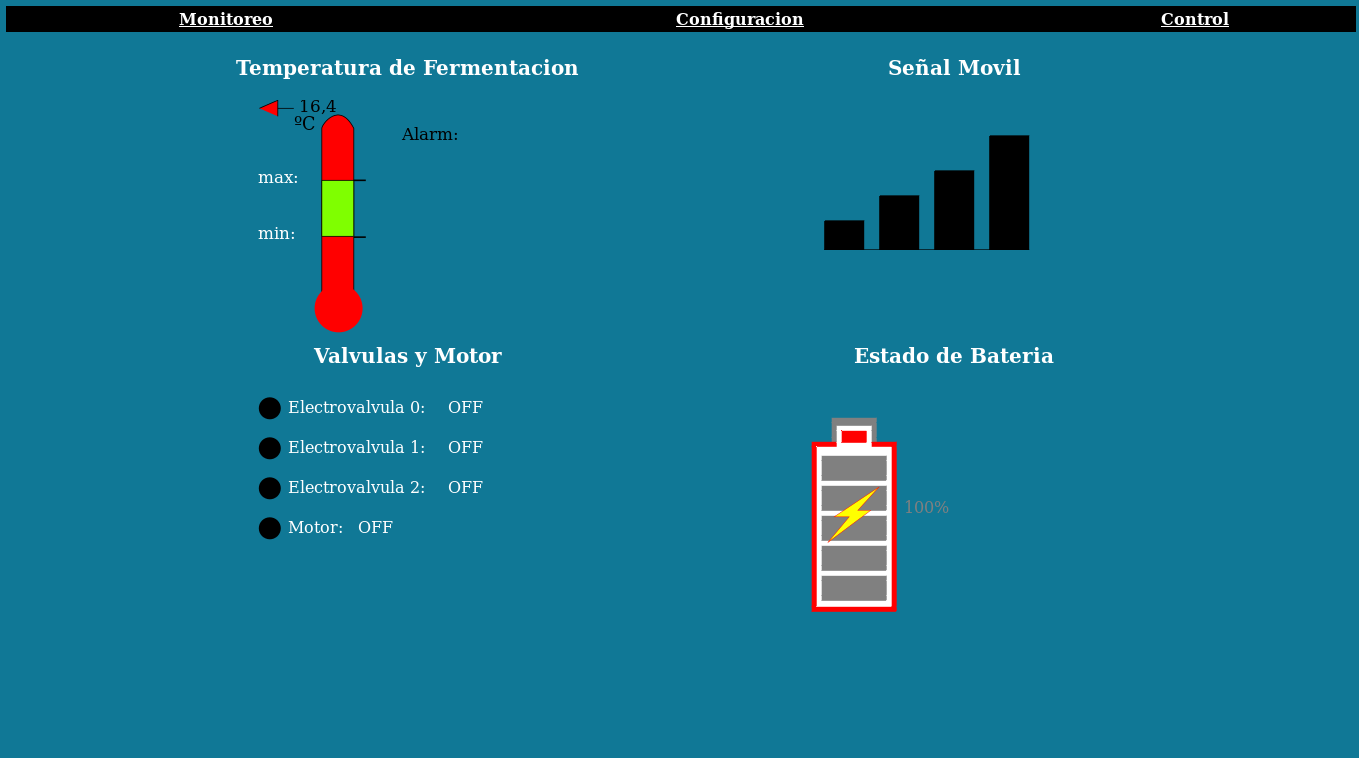
\includegraphics[scale=.25]{./Figures/old_web.png}
  \caption{Primera versión de la web de monitoreo.}
  \label{fig:old_web}
\end{figure}

Cuando ya estaba funcionando en forma correcta, se pasó a mejorar las presentación de la misma. Para ello se uso un témplate que se ajustara a las necesidades, es decir mediante un archivo que contiene un estilo ya predefinido modifica la apariencia de la web. La versión final se muestra en la figura \ref{fig:web_monitoreo}.

\begin{figure}[!h]
  \centering
  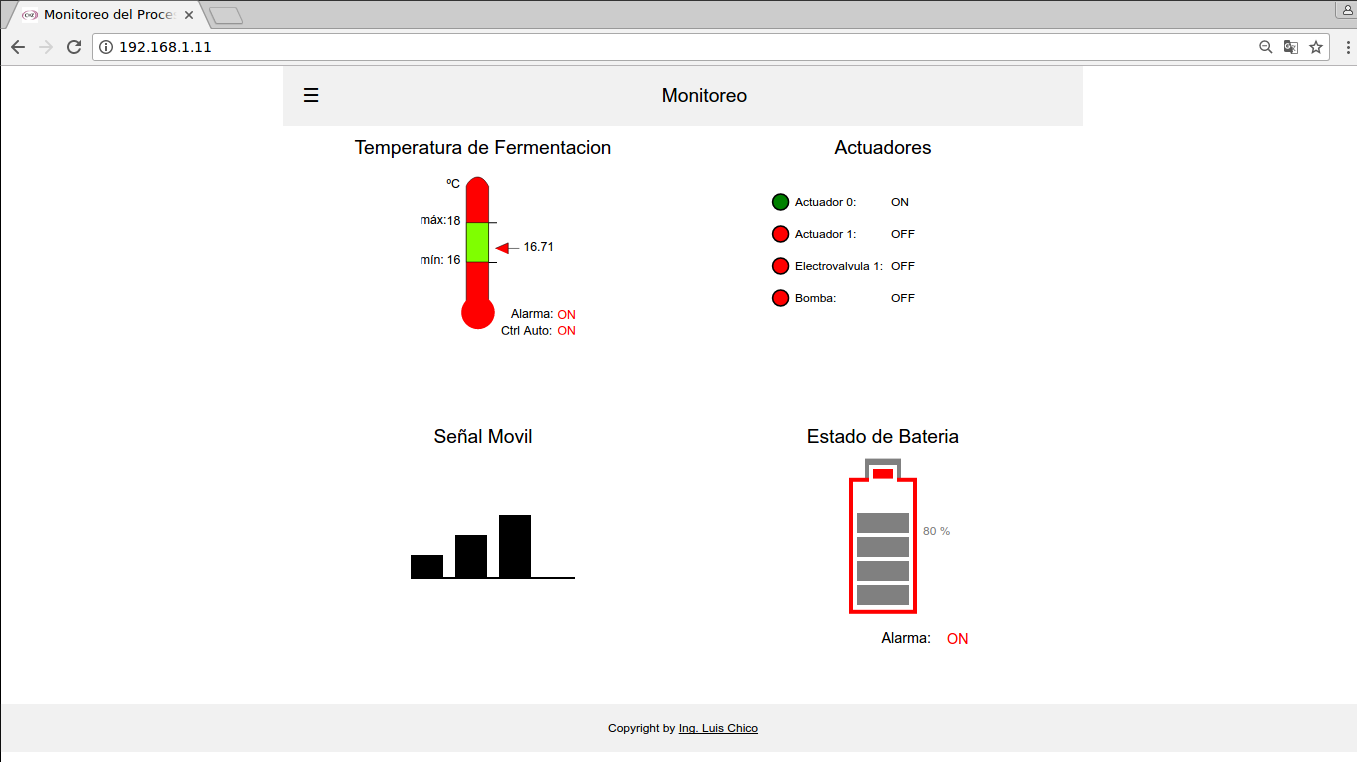
\includegraphics[scale=.25]{./Figures/web_monitoreo.png}
  \caption{Versión actualizada haciendo uso del témplate.}
  \label{fig:web_monitoreo}
\end{figure}

El template que se vió en la version final, fue encontrando en w3school\footnote{\url{https://www.w3schools.com/w3css/w3css_templates.asp}}.
Y cumplía los siguientes requerimientos:
\begin{itemize}
  \item Sea amigable.
  \item Compatible con distintos navegadores, especialmente los más utilizados como ser: Google-Chrome y Firefox. 
  \item Ser cómodo de navegar en distintos dispositivos, como tablets, celulares y PCs.
\end{itemize}


\subsection{Configuración del servidor}
Al iniciar el servidor se debe tener en cuenta que este será el encargado de gestionar las peticiones del usuario. 
Es decir una vez que el usuario ingresa la dirección del servidor, este le transmite la información de la web.
Para realizar la comunicación entre cliente y servidor se utilizó la API de lwIP \citep{webserver}  que utiliza una serie de callbacks para controlar los eventos debido a la comunicación de la red. Es por ello que para optimizar los recursos se utilizo AJAX, permitiendo que el cliente sea el encargado de realizar las consultas al server en forma periódica.

La configuración del servidor establecida por default es la que se muestra en la Tabla \ref{tab:servercfg}.
\begin{table}[!h]
  \centering
  \begin{tabular}{l c}
    \hline 
    Parámetro    & Valor \\
    \hline \hline
    IP               & 192.168.1.11 \\
    Mascara de red   & 255.255.255.0 \\
    Puerta de enlace & 192.168.0.1 \\
    Puerto           & 80 \\
    DHCP             & Deshabilitado \\
    \hline
  \end{tabular}
  \caption{Configuración por default del servidor.}
  \label{tab:servercfg}
\end{table}


La información se solicita mediante directivas del tipo SSI.
Es decir, solo se transmite un archivo ajax.shtml con los parámetros que se van a actualizar. Luego el navegador, mediante una serie de funciones en JavaScript es el encargado de actualizar los cambios realizados.  
Se puede ver el procedimiento mencionado en la figura \ref{fig:ajax_sec}.
\begin{figure}[!htb]
  \centering
  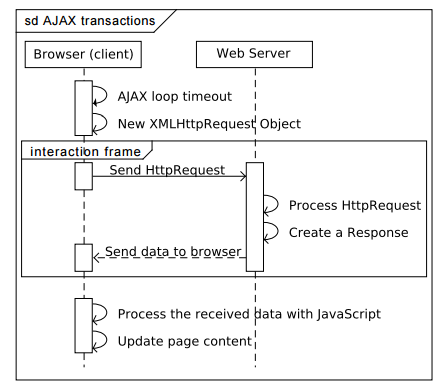
\includegraphics[scale=.8]{./Figures/ajax_sec.png}
  \caption{Diagrama de secuencia AJAX.}
  \label{fig:ajax_sec}
\end{figure}



\section{Diseño del sistema web embebido}
Se procede a navegar por el menú, figura \ref{fig:web_menus_num}, para constatar que todo el sistema esta funcionando en forma correcta. Al presionar donde dice menú, se puede configurar lo siguiente:

\begin{figure}[h]
  \centering
  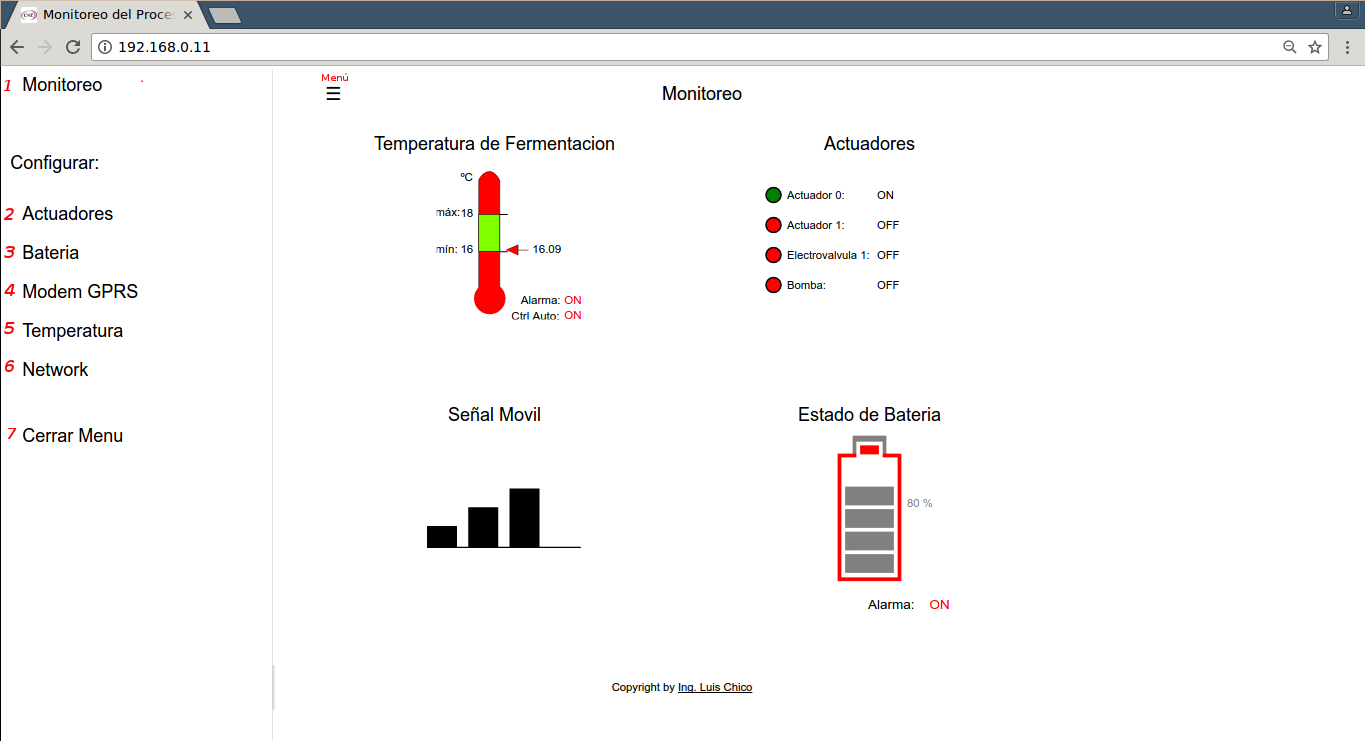
\includegraphics[scale=.25]{./Figures/web_menus_num.png}
  \caption{Opciones del al presionar sobre el menú desplegable.}
  \label{fig:web_menus_num}
\end{figure}

\begin{description}
  \item[1. Monitoreo:] Dirige a la pantalla principal, donde ver el estado del sistema. figura \ref{fig:web_monitoreo}.
  \item[2. Actuadores:] setear en forma manual el estado de los mismos. figura \ref{fig:web_act}.
  \item[3. Batería:] Aquí se podrá setear la alarma debido al nivel de descarga de batería. Esta enviará un SMS indicando que se alcanzó dicho estado. figura \ref{fig:web_bat}.
  \item[4. Módem GPRS:] En este menú podremos configurar 2 personas a quienes serán enviadas las alertas debido al accionar de alguna alarma, figura \ref{fig:web_Modem}.
  \item[5. Temperatura:] Aquí se configura el rango de temperatura, la alarma correspondiente y si se activa el control automático de la misma. De estar activado, actuará en forma automática sobre la bomba y la electroválvula para mantener la temperatura dentro de dicho rango. figura \ref{fig:web_temp}.
  \item[6. Network:] Aquí se configura los parámetros de la red, IP, mascara de red y puerta de enlace. figura \ref{fig:cfg_net}.
  \item[7. Cerrar Menú:] Esta opción cierra el menú, permitiendo quitar las opciones de menú.
\end{description}

\begin{figure}[h]
  \centering
  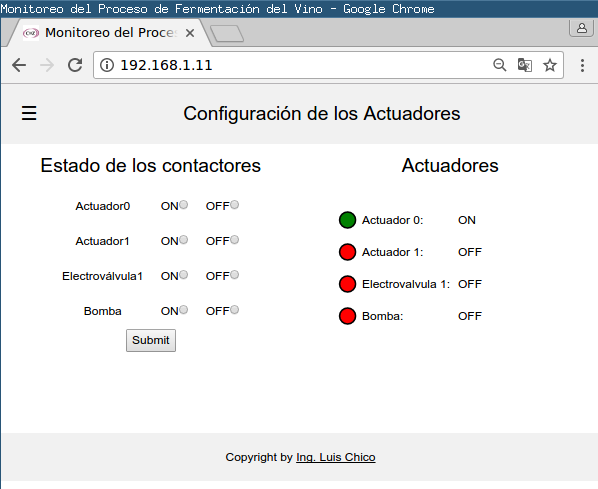
\includegraphics[scale=.35]{./Figures/config_act.png}
  \caption{ Activar/Desactivar actuadores.}
  \label{fig:web_act}
\end{figure}

\begin{figure}[h]
  \centering
  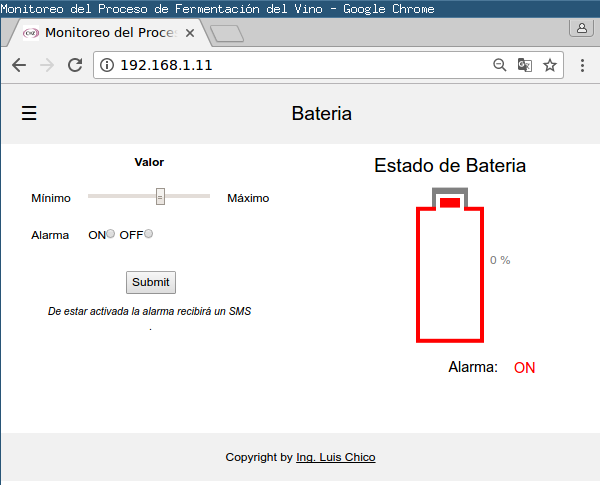
\includegraphics[scale=.35]{./Figures/config_bat.png}
  \caption{Configurar nivel de descarga para accionar la alerta por batería baja.}
  \label{fig:web_bat}
\end{figure}
\begin{figure}[h]
  \centering
  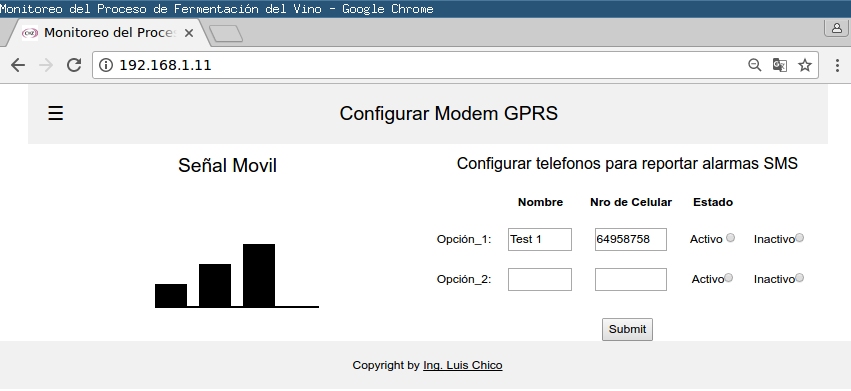
\includegraphics[scale=.35]{./Figures/config_Modem.png}
  \caption{Configuración de los celulares.}
  \label{fig:web_Modem}
\end{figure}
\begin{figure}[h]
  \centering
  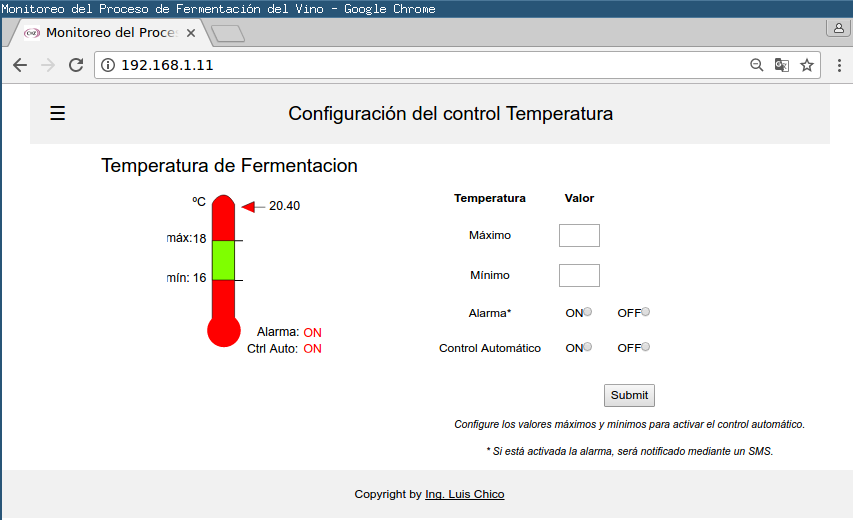
\includegraphics[scale=.35]{./Figures/config_temp.png}
  \caption{Configuración del rango de temperatura y activación del estado de control automático y alarma.}
  \label{fig:web_temp}
\end{figure}
\begin{figure}[h]
  \centering
  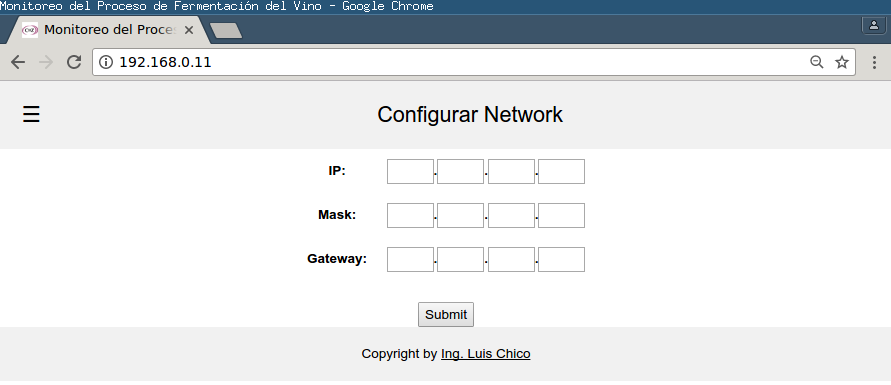
\includegraphics[scale=.35]{./Figures/config_network.png}
  \caption{Configuración de IP, mascara de red y puerta de enlace.}
  \label{fig:cfg_net}
\end{figure}











%\begin{verbatim}
%\begin{lstlisting}[caption= "un epígrafe descriptivo"]
%
%	las líneas de código irían aquí...
%	
%\end{lstlisting}
%\end{verbatim}
%
%A modo de ejemplo:
%
%\begin{lstlisting}[caption=Pseudocódigo del lazo principal de control.]  % Start your code-block
%
%#define MAX_SENSOR_NUMBER 3
%#define MAX_ALARM_NUMBER  6
%#define MAX_ACTUATOR_NUMBER 6
%
%uint32_t sensorValue[MAX_SENSOR_NUMBER];		
%FunctionalState alarmControl[MAX_ALARM_NUMBER];	//ENABLE or DISABLE
%state_t alarmState[MAX_ALARM_NUMBER];						//ON or OFF
%state_t actuatorState[MAX_ACTUATOR_NUMBER];			//ON or OFF
%
%void vControl() {
%
%	initGlobalVariables();
%	
%	period = 500 ms;
%		
%	while(1) {
%
%		ticks = xTaskGetTickCount();
%		
%		updateSensors();
%		
%		updateAlarms();
%		
%		controlActuators();
%		
%		vTaskDelayUntil(&ticks, period);
%	}
%}
%\end{lstlisting}
%


